Im Folgenden sind die während des Versuchs aufgenommenen Daten und die aus diesen
berechneten Größen tabellarisch aufgetragen. An entsprechender Stelle sind Erklärungen
zu den Werten und Berechnungen gegeben.\\

In \autoref*{tab:Daten} befinden sich die für die Auswertung verwendeten Messdaten für die Temperaturen
$T_{1}\ \text{und}\ T_{2}$, die Drücke $p_{b}\ \text{und}\ p_{a}$, sowie die Zeit $t$ der Aufnahme nach Beginn des Versuchs.as

\begin{table}
\centering
\begin{tabular}{|r|C|C|C|C|}
	\hline
	         Zeit & {Temperatur}       & {Druck}             & {Temperatur}       & {Druck}             \\
	$t\,[\si{s}]$ & $T_{1}\,[\si{°C}]$ & $p_{b}\,[\si{bar}]$ & $T_{2}\,[\si{°C}]$ & $p_{a}\,[\si{bar}]$ \\ \hline\hline
	            0 & \num{26,6(1)}      & \num{7,0(5)}        & \num{17,4(1)}      & \num{4,6(2)}        \\
	           90 & \num{28,0(1)}      & \num{7,5(5)}        & \num{16,5(1)}      & \num{4,6(2)}        \\
	          180 & \num{30,1(1)}      & \num{7,9(5)}        & \num{15,1(1)}      & \num{4,4(2)}        \\
	          270 & \num{32,1(1)}      & \num{8,0(5)}        & \num{13,9(1)}      & \num{4,2(2)}        \\
	          360 & \num{34,0(1)}      & \num{8,5(5)}        & \num{12,7(1)}      & \num{4,1(2)}        \\
	          450 & \num{35,2(1)}      & \num{9,0(5)}        & \num{11,9(1)}      & \num{4,0(2)}        \\
	          540 & \num{37,0(1)}      & \num{9,0(5)}        & \num{10,9(1)}      & \num{4,0(2)}        \\
	          630 & \num{38,6(1)}      & \num{9,5(5)}        & \num{9,8(1)}       & \num{3,9(2)}        \\
	          720 & \num{40,2(1)}      & \num{10,0(5)}       & \num{8,9(1)}       & \num{3,9(2)}        \\
	          810 & \num{41,7(1)}      & \num{10,0(5)}       & \num{8,0(1)}       & \num{3,8(2)}        \\
	          900 & \num{43,1(1)}      & \num{10,5(5)}       & \num{7,2(1)}       & \num{3,6(2)}        \\
	          990 & \num{44,5(1)}      & \num{11,0(5)}       & \num{6,5(1)}       & \num{3,6(2)}        \\
	         1080 & \num{45,8(1)}      & \num{11,0(5)}       & \num{5,9(1)}       & \num{3,6(2)}        \\
	         1170 & \num{46,6(1)}      & \num{11,5(5)}       & \num{5,4(1)}       & \num{3,6(2)}        \\
	         1260 & \num{47,9(1)}      & \num{12,0(5)}       & \num{4,9(1)}       & \num{3,6(2)}        \\
	         1350 & \num{49,0(1)}      & \num{12,0(5)}       & \num{4,4(1)}       & \num{3,5(2)}        \\ \hline
\end{tabular}
\caption{Messwerte der Temperaturen und Drücke}
\label{tab:Daten}
\end{table}

In \autoref{fig:T1} \ref{fig:T2} sind die Temperaturverläufe für $T_{1}$ und $T_{2}$ jeweils mit der entsprechenden 
Regressionskurve dargestellt.
Die mit Hilfe der Python Bibliothek \emph{SciPy} bestimmten Regressionsparameter für die Kurven der Form
$T(t) = At^{2} + Bt + C$ sind in \autoref{tab:Param} gelistet.

\begin{table}[!h]
  	\centering
   	\begin{tabular}{|c||c|c|c|}
   		\hline
   		Funktion & A& B& C\\ \hline \hline
   		$T_{1}$& \num{-3.87(29)e-06}& \num{2.20(4)e-04}& \num{299.49(12)}\\
    		$T_{2}$& \num{3.59(20)e-06}& \num{-1.47(3)e-02}& \num{290.76(9)}\\
    		\hline
   	\end{tabular}
   	\label{tab:Param}
   	\caption{Parameter der Regression mit $T(t) = At^{2} + Bt + C$ }
\end{table}
	
\begin{figure}
	\centering
	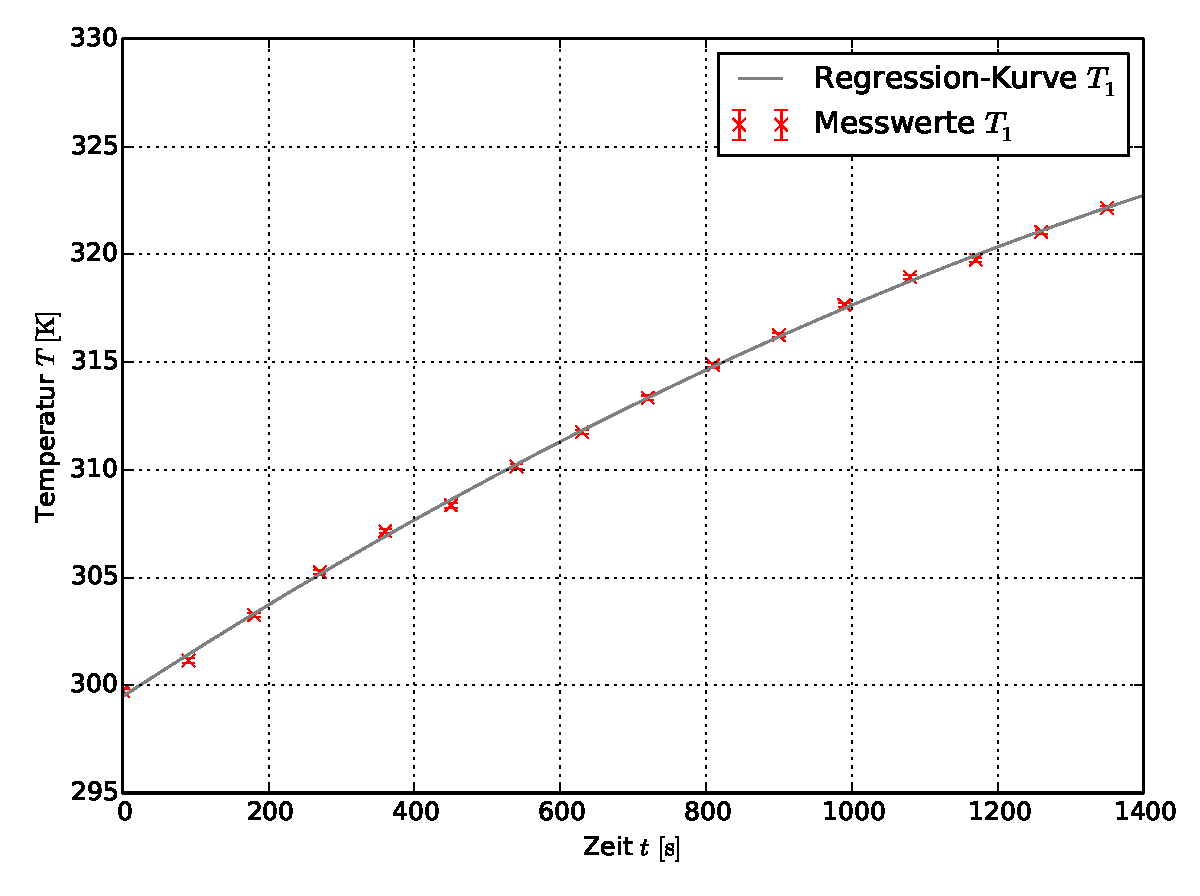
\includegraphics[scale=0.75]{Plots/Temperaturverlauf_T1.pdf}
 	\caption{Temperaturverlauf mit Regressionskurve von $T_{1}$}
 	\label{fig:T1}
\end{figure}

\begin{figure}
	\centering
	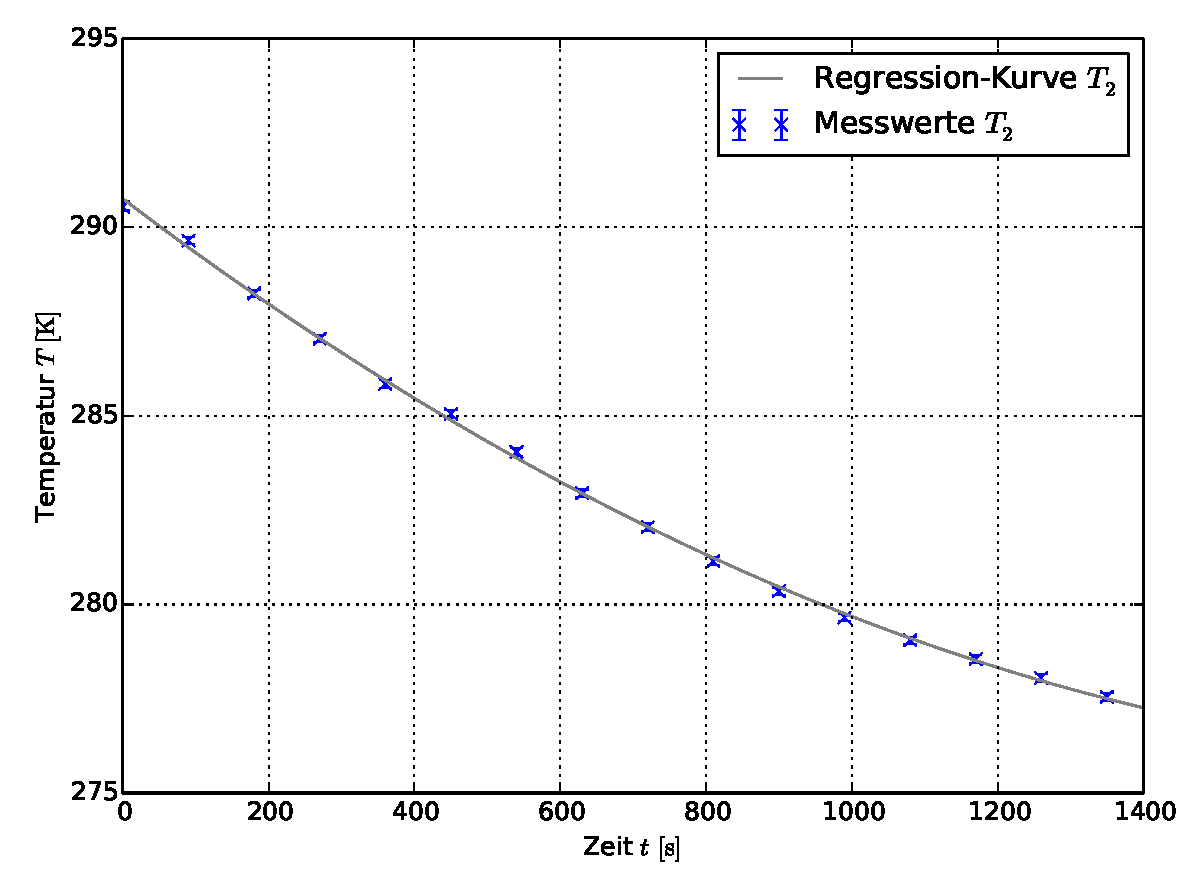
\includegraphics[scale=0.75]{Plots/Temperaturverlauf_T2.pdf}
	\caption{Temperaturverlauf mit Regressionskurve von $T_{2}$}
	\label{fig:T2}
\end{figure}

Aus den Regressionskurven für die Temperaturverläufe lassen sich nun deren Differentialquotienten $\od{T_{1}}{t}$ und $\tod{T_{2}}{t}$
bestimmen, durch die, die gesuchten Apparaturgrößen berechnet werden können. Die Differntialqoutienten $\od{T_{1}}{t}$ und die 
berechneten, idealen und realen, Güteziffern sowie deren relativer Unterschied sind in \autoref{tab:Güte}, die 
Differnetialquotienten $\od{T_{2}}{t}$ und der daraus bestimmte Massendurchsatz des Transportgases $\tfrac{\Delta m}{\Delta t}$
in \autoref{tab:Masse} zu finden.

Die Berechnung der idealen Güteziffer erfolgt nach \eqref{eq:vid} durch einsetzen der Temperaturen $T_{1}$ und $T_{2}$ zu den entsprechnden
Zeiten. 	

\begin{table}
	\centering
	\begin{tabular}{|c|c|c|c|c|}
		\hline
		    Zeit      &    Differentialquotient    & reale Güteziffer  & ideale Güteziffer &     relativer Unterschied     \\
		$t\,[\si{s}]$ & $\od{T_{1}}{t}\,[Ks^{-1}]$ & $\nu_{real}\,[1]$ &  $\nu_{id}\,[1]$  & $\frac{\nu_{real}}{\nu_{id}}$ \\ \hline\hline
		     180      &        \num{0.021}         & \num{2.879(115)}  & \num{20.217(186)} &          \num{0.142}          \\
		     360      &        \num{0.019}         & \num{2.684(107)}  & \num{14.420(093)} &          \num{0.186}          \\
		     540      &        \num{0.018}         & \num{2.490(100)}  & \num{11.883(062)} &          \num{0.210}          \\
		     720      &        \num{0.017}         & \num{2.296(092)}  & \num{10.011(043)} &          \num{0.229}          \\ \hline
	\end{tabular}
	\caption{Reale und ideale Güteziffer im Verhältnis}
	\label{tab:Güte}
\end{table}

\begin{table}
	\centering
	\begin{tabular}{|c|c|c|c|}
		\hline
		    Zeit      &    Differentialquotient    &               Massendurchsatz                & Mechanische Leistung \\
		$t\,[\si{s}]$ & $\od{T_{2}}{t}\,[Ks^{-1}]$ & $\tfrac{\Delta m}{\Delta t}\,[\si{gs^{-1}}]$ & $P_{mech}\,[\si{W}]$ \\ \hline\hline
		     180      &        \num{-0.013}        &               \num{1.479(39)}                &  \num{15.075(396)}   \\
		     360      &        \num{-0.012}        &               \num{1.336(35)}                &  \num{16.976(446)}   \\
		     540      &        \num{-0.011}        &               \num{1.193(31)}                &  \num{16.843(443)}   \\
		     720      &        \num{-0.010}        &               \num{1.050(28)}                &  \num{17.234(453)}   \\ \hline
	\end{tabular}
	\caption{Massendurchsatz des Transportgases}
	\label{tab:Masse}
\end{table}




		